% Guía explicativa de la tesis para el autor. Compilar desde informe/:  ./tectonic.exe guia_explicativa.tex
\documentclass[11pt,a4paper]{article}
\usepackage{fontspec}
\usepackage[spanish,es-nodecimaldot,es-noshorthands,es-tabla]{babel}
\usepackage[margin=2.3cm]{geometry}
\usepackage{amsmath,amssymb}
\usepackage{graphicx,booktabs,tabularx,array,float,enumitem}
\usepackage[font=small,labelfont=bf]{caption}
\usepackage[most]{tcolorbox}
\usepackage[hidelinks]{hyperref}
\graphicspath{{../notebooks/resultados/figuras/}}
\setlength{\parskip}{0.45em}\setlength{\parindent}{0pt}
\linespread{1.12}

\definecolor{azul}{HTML}{1F3A5F}
\definecolor{fondo}{HTML}{EEF3F9}
\definecolor{ambar}{HTML}{FFF4DC}
\newtcolorbox{idea}[1]{colback=fondo,colframe=azul,fonttitle=\bfseries,title=#1,boxrule=0.6pt,arc=2pt}
\newtcolorbox{ojo}[1]{colback=ambar,colframe=orange!70!black,fonttitle=\bfseries,title=#1,boxrule=0.6pt,arc=2pt}
\newcolumntype{L}{>{\raggedright\arraybackslash}X}

\title{\color{azul}\textbf{Guía explicativa de la tesis}\\[4pt]\large Del análisis exploratorio al machine learning causal\\ qué se hizo, cómo y por qué}
\author{Luis Azaña}
\date{Octubre 2026}

\begin{document}
\maketitle

\begin{idea}{Cómo leer esta guía}
Está escrita para alguien que ya domina EDA, análisis de datos y machine learning, pero no tanto la estadística ni la inferencia causal. Cada concepto estadístico se explica la primera vez que aparece, y al final hay un glosario (sección~\ref{sec:glosario}). Las cifras son las de las ejecuciones finales de los notebooks~2, 2b, 3, 3b y~4 (muestra con direcciones exactas, cochera como tratamiento principal).
\end{idea}

\tableofcontents
\newpage

% =====================================================================
\section{Qué se quiere lograr}

\subsection{La pregunta}

La tesis responde una pregunta de \textbf{causa y efecto}:

\begin{center}
\large\itshape ¿Cuánto cambiaría el precio de alquiler de un departamento\\ si incluyera cochera, sin cambiar nada más?
\end{center}

Como \textbf{análisis secundario} se repite la pregunta para \emph{un baño adicional}, que era la pregunta del entregable anterior.

\subsection{Por qué es difícil: el problema de la confusión}

Los departamentos con cochera incluida también son más grandes (96 frente a 65\,m²), tienen más baños y están en los distritos más caros. Si se comparan directamente, se mezcla el efecto de la cochera con el de todo lo demás.

\begin{idea}{Ejemplo intuitivo}
Las personas que usan encendedor tienen más cáncer de pulmón. ¿El encendedor causa cáncer? No: fumar causa ambas cosas. Fumar es un \textbf{confusor}. En la tesis, la \textbf{ubicación} y el \textbf{área} cumplen ese papel: causan a la vez ``tener cochera'' y ``costar más''.
\end{idea}

Con los datos de la tesis:
\begin{itemize}
\item Comparación directa: los departamentos con cochera incluida cuestan \textbf{63\,\%} más.
\item Efecto aislado (resultado final): \textbf{7.5\,\%}.
\end{itemize}

\subsection{Dos problemas extra de esta versión}

\begin{enumerate}
\item \textbf{La cochera no está en la base.} Hay que leerla en el texto del aviso. Para eso se usa IA (OpenAI), con cuidado de no gastar de más y de medir sus errores.
\item \textbf{No todas las ubicaciones son exactas.} Google devuelve la precisión de cada dirección. Solo \texttt{ROOFTOP} es el edificio exacto; las demás pueden errar por cientos de metros. Como la ubicación es el confusor más importante, \textbf{solo se usan direcciones \texttt{ROOFTOP}}.
\end{enumerate}

\subsection{Por qué no basta con un buen modelo de machine learning}

Un modelo predictivo responde \emph{``¿cuánto costará este departamento?''}. La importancia de una variable (o su valor SHAP) dice \emph{cuánto la usa el modelo para adivinar}, no \emph{qué pasaría si la cambiaras}.

\begin{ojo}{La idea central de tu asesor}
``No se declara identificada una relación causal por usar XGBoost, redes o DML.'' La causalidad viene de \textbf{supuestos explícitos} (qué causa qué), que luego se ponen a prueba.
\end{ojo}

\subsection{Objetivos e hipótesis}

\textbf{Objetivo general:} estimar el efecto causal de que un departamento incluya cochera sobre su precio de oferta y evaluar qué tan sólido es.

\begin{table}[H]\small
\caption{Objetivos específicos (los define tu asesor en \texttt{nuevo\_informe})}
\begin{tabularx}{\textwidth}{lLl}
\toprule
Objetivo & Qué pregunta responde & Estado \\
\midrule
OE1 Auditar los datos & ¿Sobre qué población valen los resultados? & Hecho \\
OE2 Identificación & ¿Qué variables controlar y por qué? (DAG) & Hecho \\
OE3 Estimación & ¿Cuánto vale la cochera? ¿Cómo se compara con la regresión? & Hecho \\
OE4 Variación y sensibilidad & ¿Cambia con otras decisiones? ¿Varía por zona? ¿Qué tan frágil es? & Hecho \\
OE5 IA sobre el texto & ¿Se puede medir la cochera desde la descripción? & Hecho (falta validación humana) \\
OE6 Simulación & ¿El método funciona cuando conozco la respuesta? & Hecho \\
OE7 Trazabilidad & ¿Se puede reproducir cada número? & Parcial \\
\bottomrule
\end{tabularx}
\end{table}

\begin{description}[leftmargin=1cm]
\item[H1] Ajustar por los confusores cambia de forma clara la asociación inicial.
\item[H2] Elegir bien los controles importa más que elegir el algoritmo.
\item[H3] El efecto varía por zona o por tamaño (solo si la precisión lo permite).
\item[H4] La conclusión depende de cuán fuertes sean los factores no observados.
\end{description}

% =====================================================================

\section{Qué dice el notebook de análisis y pruebas estadísticas}

Esta sección resume \texttt{notebook0} y \texttt{notebook1} (el trabajo previo) y explica qué hace cada prueba estadística.

\subsection{Preparación y EDA}
\begin{itemize}
\item \texttt{notebook0} toma 3\,739 avisos del scraping, quita los que no tienen dormitorios, baños, área, precio o distrito (quedan 3\,516) y crea variables: precio por m², fecha de publicación binaria y grupos de antigüedad.
\item \texttt{notebook1} elimina atípicos (precio por m² extremo, combinaciones raras de dormitorios y baños, precios menores de S/\,600) y queda con \textbf{3\,276 avisos}.
\item \textbf{Clustering} (K-means sobre PCA de dormitorios, baños, área y precio; 89\,\% de la varianza en 2 componentes): tres tipos de departamento, pequeños (unos 56\,m², S/\,2\,100), ``normales'' (unos 94\,m², S/\,2\,860) y amplios (unos 238\,m², S/\,8\,140).
\item \textbf{Correlaciones}: precio y área tienen una correlación de 0.83. Barranco, Miraflores, San Isidro y Lince tienen el precio por m² más alto.
\end{itemize}

\subsection{Las pruebas estadísticas, explicadas}

\begin{idea}{Qué es un p-valor (en una frase)}
Es la probabilidad de ver una diferencia tan grande como la observada \emph{si en realidad no hubiera ninguna diferencia}. Si es menor que 0.05, se dice que la diferencia es ``estadísticamente significativa'': es poco probable que sea solo azar. No dice nada sobre causas.
\end{idea}

\begin{table}[H]\small
\caption{Las 8 aseveraciones del \texttt{notebook1} (valores de sus salidas actuales)}
\begin{tabularx}{\textwidth}{>{\raggedright\arraybackslash}p{3.2cm}>{\raggedright\arraybackslash}p{3.6cm}L}
\toprule
Aseveración & Prueba (qué hace) & Resultado \\
\midrule
1. Precio/m² entre distritos top & \textbf{Tukey}: compara las medias de varios grupos de dos en dos, corrigiendo por hacer muchas comparaciones & Barranco es el más caro; Miraflores está por encima de San Isidro y Lince; San Isidro y Lince no difieren ($p=0.43$) \\
2. Medianas Miraflores, San Isidro y Lince & \textbf{Kruskal-Wallis}: compara grupos usando rangos (no supone distribución normal) & $p=0.006$: las medianas no son iguales (Miraflores es mayor) \\
3. Lima Top al menos 30\,\% más caro por m² & \textbf{Prueba t}: compara las medias de dos grupos & Diferencia estimada del 36\,\%, $p=0.0007$ \\
4. Antigüedad y precio & \textbf{Spearman}: correlación por rangos (mide si una variable sube cuando la otra sube, aunque no sea en línea recta) & $\rho=0.07$: relación positiva muy débil \\
5. Antigüedad y área & Spearman & $\rho=0.31$: los departamentos antiguos son más grandes \\
6. Antigüedad y precio/m² & Spearman & $\rho=-0.34$: los antiguos son más baratos por m² \\
7. Antigüedad y dormitorios + baños & Spearman & $\rho=0.19$: los antiguos tienen más ambientes \\
8. Distribución interna y precio, controlando el área & \textbf{Regresión lineal múltiple} por clase de distrito & A igual área: un baño más se asocia con S/\,195--298 más y un dormitorio más con S/\,168--323 menos ($R^2=0.62$--$0.74$) \\
\bottomrule
\end{tabularx}
\end{table}

\subsection{Qué aporta y qué no aporta este análisis}

\textbf{Aporta} una descripción sólida del mercado: dónde es caro, cómo se relacionan tamaño, antigüedad y precio, y qué tipos de departamento existen. Todo eso se reutiliza para \emph{construir el modelo causal}: por ejemplo, la aseveración 5 (los antiguos son más grandes) justifica la flecha ``antigüedad $\rightarrow$ área'' del grafo.

\textbf{No aporta} efectos causales:
\begin{itemize}
\item Las pruebas 1--7 comparan grupos o correlacionan dos variables \emph{sin controlar nada más}. Que Lima Top sea un 36\,\% más caro por m² puede deberse, en parte, a que allí los departamentos son distintos.
\item La aseveración 8 sí intenta ``controlar el área'' y, por eso, \textbf{es la semilla de la tesis actual}. Pero usa una regresión lineal con variables elegidas a mano: no justifica por qué esas variables y no otras, supone relaciones en línea recta y trata cada aviso como independiente.
\end{itemize}

\begin{idea}{Conexión clave}
La aseveración 8 ya era una pregunta causal (``el efecto de los baños, a igual área'') resuelta con herramientas asociativas. La tesis actual responde \emph{la misma pregunta} con las herramientas correctas: grafo causal, Double ML, inferencia agrupada, análisis de sensibilidad y simulación.
\end{idea}

% =====================================================================
\section{Qué se hace luego: el análisis causal paso a paso}

El flujo nuevo tiene cinco notebooks, en este orden:

\begin{center}\small
\texttt{notebook2\_auditoria} $\rightarrow$ \texttt{notebook2b\_extraccion\_ia} $\rightarrow$ \texttt{notebook3b\_efecto\_cochera}\\
$\rightarrow$ \texttt{notebook3\_estimacion\_causal} (baños) $\rightarrow$ \texttt{notebook4\_semisintetico}
\end{center}

Las funciones comunes están en \texttt{causal\_utils.py}, \texttt{extraccion\_ia.py} y \texttt{semisintetico.py}.

\subsection{Paso 1 --- Auditoría de los datos (notebook 2)}

\begin{table}[H]\small
\caption{De dónde salen los 2\,220 avisos finales}
\begin{tabularx}{\textwidth}{Lrr}
\toprule
Paso & Excluidos & Quedan \\
\midrule
Archivo crudo del scraping & -- & 3\,739 \\
Sin baños, dormitorios, área, precio o distrito & 223 & 3\,516 \\
Duplicados (83 eran el mismo aviso en dos distritos) & 243 & 3\,273 \\
Coordenada a más de 8\,km de su distrito & 26 & 3\,247 \\
\textbf{Dirección no exacta} (distinta de \texttt{ROOFTOP}) & 967 & 2\,280 \\
Reglas del \texttt{notebook1} (rangos, combinaciones raras, atípicos) & 60 & \textbf{2\,220} \\
\bottomrule
\end{tabularx}
\end{table}

\begin{idea}{Qué es ROOFTOP}
Cuando Google geocodifica una dirección, devuelve su precisión. \texttt{ROOFTOP} es el edificio exacto. \texttt{RANGE\_INTERPOLATED} está interpolada en la cuadra, \texttt{GEOMETRIC\_CENTER} es el centro de una calle y \texttt{APPROXIMATE} el centro del barrio, donde caen decenas de avisos en el mismo punto. Solo el 70\,\% de los avisos era \texttt{ROOFTOP}.
\end{idea}

\subsection{Paso 2 --- Medir la cochera con IA (notebook 2b)}

Para ahorrar tokens, la extracción se hace en capas:
\begin{enumerate}
\item \textbf{Regex}: se buscan \emph{cochera, estacionamiento, parqueo, parking, garaje} y sus variantes. Si no aparece ninguna, el aviso queda como \emph{sin cochera} \textbf{sin llamar a la API} (659 avisos).
\item \textbf{Fragmento}: para cada mención en la posición $x$ se toma \texttt{texto[x-200 : x+200]} (sin pasarse de los bordes). Los fragmentos que se tocan se unen.
\item \textbf{Privacidad}: se borran teléfonos, correos y enlaces.
\item \textbf{OpenAI}: \texttt{gpt-4.1-mini-2025-04-14}, temperatura 0, respuesta obligada a un JSON fijo:
\begin{center}\small\texttt{\{"cochera":"si", "tipo":"incluida", "precio\_extra":0, ..., "motivo":"Incluye 1 estacionamiento"\}}\end{center}
\item \textbf{Caché}: cada respuesta se guarda; volver a ejecutar no cuesta nada.
\end{enumerate}

Un \textbf{piloto de 25 avisos} reveló tres errores del primer prompt: marcar como ``ambigua'' una cochera sin precio, leer ``ALQUILER CON COCHERA \$700'' como 700 de costo extra y no reconocer ``sin cochera, pero se puede alquilar''. Se corrigieron antes de la corrida completa. \textbf{Costo total: 0.76 USD.}

\begin{table}[H]\small
\caption{Resultado de la extracción}
\begin{tabularx}{\textwidth}{Lrl}
\toprule
Clasificación & N & Uso \\
\midrule
Cochera incluida (sin pago extra mencionado) & 1\,095 & $D=1$ \\
No menciona cochera & 659 & $D=0$ \\
Menciona, pero la IA lee ``no tiene'' (visitas, calle, ``sin cochera'') & 297 & $D=0$ \\
Cochera con costo extra (mediana S/\,250) & 150 & Excluido \\
Ambigua & 19 & Excluido \\
\bottomrule
\end{tabularx}
\end{table}

\begin{ojo}{Supuestos de esta medición}
(1) Si el aviso no menciona cochera, se asume que no la tiene. (2) Si tiene cochera y no menciona un pago extra, se asume incluida. Solo 155 avisos dicen ``incluida'' literalmente. (3) Tu asesor exige una \textbf{validación humana}: hay 249 avisos listos para que los etiquetes en \texttt{csv/validacion\_cochera\_para\_etiquetar.csv}.
\end{ojo}

\subsection{Paso 3 --- El grafo causal (DAG)}

\begin{figure}[H]
\centering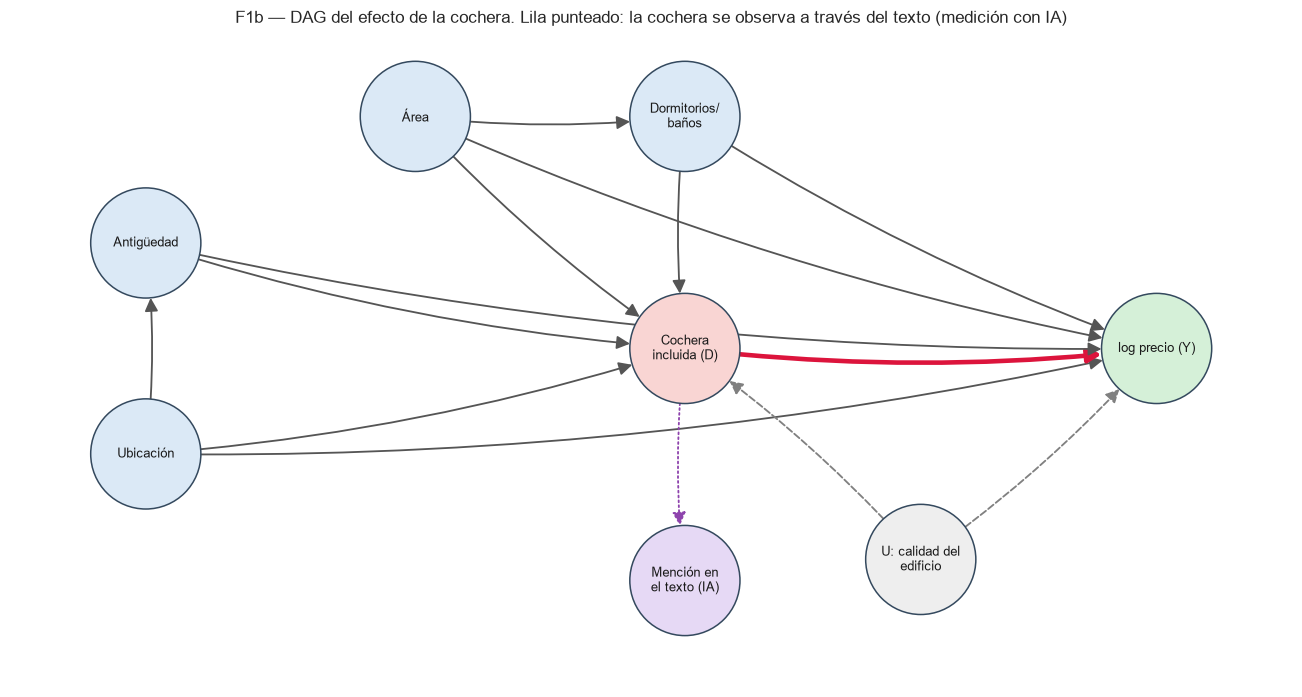
\includegraphics[width=0.9\textwidth]{F1b_dag_cochera.png}
\caption{DAG de la cochera. La flecha roja es el efecto que se quiere medir.}
\end{figure}

\begin{table}[H]\small
\caption{Tipos de variables y qué hacer con cada una}
\begin{tabularx}{\textwidth}{>{\raggedright\arraybackslash}p{2.6cm}>{\raggedright\arraybackslash}p{3.6cm}>{\raggedright\arraybackslash}p{1.8cm}L}
\toprule
Tipo & Forma en el grafo & ¿Controlar? & En la tesis \\
\midrule
\textbf{Confusor} & Causa a D y a Y & \textbf{Sí} & Área, ubicación, antigüedad, baños, dormitorios \\
\textbf{Descendiente de Y} & Consecuencia del resultado & \textbf{No} & Precio por m² \\
\textbf{Confusor no observado} & Causa a D y a Y, no está en los datos & Imposible & Calidad del edificio \\
\bottomrule
\end{tabularx}
\end{table}

El grafo no lo deciden los datos: lo construyes tú con conocimiento del mercado y con el \textbf{orden temporal}. Primero existen el terreno y el edificio, luego se diseña el departamento (con o sin cochera) y al final se fija el precio. Las flechas no tienen peso; solo dicen qué controlar.

\subsection{Paso 4 --- Qué se estima (el ``estimando'')}

El \textbf{efecto promedio} (ATE) de tener cochera incluida, en log del precio, entre los avisos con \textbf{soporte común}. En porcentaje es $100\,(e^\theta-1)$.

\begin{idea}{Propensión y soporte común}
La \textbf{propensión} $m(X)$ es la probabilidad de que un aviso tenga cochera dado su perfil (área, zona\ldots). Si un perfil tiene propensión 0.99, casi todos los departamentos parecidos tienen cochera: no hay con quién compararlo. El \textbf{soporte común} es quedarse con los avisos con propensión entre 0.05 y 0.95, donde sí hay comparaciones reales.
\end{idea}

\subsection{Paso 5 --- Double ML interactivo (dónde está el ML)}

Como el tratamiento es sí/no, se usa la versión \textbf{IRM} (o AIPW) de Double ML, con \textbf{3 modelos} de \textit{gradient boosting}:
\begin{enumerate}
\item \textbf{Modelo A} (clasificador): predice si tiene cochera a partir de $X$. Es la propensión $\hat m(X)$.
\item \textbf{Modelo B}: predice el precio \emph{de los que tienen cochera} a partir de $X$, $\hat g_1(X)$.
\item \textbf{Modelo C}: predice el precio \emph{de los que no tienen}, $\hat g_0(X)$.
\end{enumerate}
Para cada aviso se calcula el \textbf{score doblemente robusto}:
\[
\phi=\underbrace{\hat g_1-\hat g_0}_{\text{diferencia predicha}}+\underbrace{\frac{D\,(Y-\hat g_1)}{\hat m}-\frac{(1-D)\,(Y-\hat g_0)}{1-\hat m}}_{\text{corrección por el error de predicción}}
\]
El efecto es el \textbf{promedio de $\phi$} en el soporte común. ``Doblemente robusto'' significa que basta con que el modelo de la propensión \emph{o} el del precio esté bien para que el resultado sea correcto.

\textbf{Igual que antes}: \textit{cross-fitting} con 5 folds agrupados por edificio (un edificio nunca está a la vez en entrenamiento y en prueba), 10 repeticiones y errores agrupados por edificio.

\begin{idea}{Balance: ¿quedaron comparables?}
Se mide la \textbf{diferencia estandarizada} (SMD) de cada variable entre los grupos con y sin cochera. Antes del ajuste, el área difiere 0.92 desviaciones estándar; después de ponderar por la propensión, todas quedan por debajo de 0.05. Bajo 0.1 se considera buen balance.
\end{idea}

\subsection{Paso 6 --- Grilla, sensibilidad, grupos y espacio}

\begin{itemize}
\item \textbf{Grilla}: se repite cambiando \emph{una} decisión (quitar la ubicación, agregar el precio/m², usar la definición estricta de ``incluida'', etc.).
\item \textbf{Sensibilidad}: ¿qué tan fuerte tendría que ser un factor oculto (la calidad del edificio) para anular el efecto? Se compara con la fuerza de los factores observados.
\item \textbf{GATE}: el efecto por clase de distrito y por tamaño, con una prueba de Wald de igualdad.
\item \textbf{I de Moran}: ¿los errores de avisos cercanos se parecen?
\end{itemize}

\subsection{Paso 7 --- Baños (notebook 3) y simulación (notebook 4)}

\begin{itemize}
\item \textbf{Baños}: el mismo análisis del entregable anterior (Double ML parcialmente lineal: 2 modelos y residuos), ahora solo con ROOFTOP y con la cochera como control adicional.
\item \textbf{Simulación}: se toman los avisos reales y se \emph{inventa} el tratamiento y el precio con un efecto conocido (0.10 para la cochera, 0.05 para los baños), con y sin factores ocultos. Se mide si los métodos aciertan. Son 800 réplicas en total.
\end{itemize}

% =====================================================================
\section{Resultados y cómo responden a lo que pide tu asesor}

\subsection{Resultado principal (OE3, H1)}

\begin{table}[H]\small
\caption{Efecto de tener cochera incluida}
\begin{tabularx}{\textwidth}{Lrcr}
\toprule
Método & Efecto & IC 95\,\% & En soles (alquiler S/\,2\,650) \\
\midrule
Diferencia directa & 63.0\,\% & 56.8 -- 69.4\,\% & S/\,1\,668 \\
Regresión lineal con controles & 7.8\,\% & 5.0 -- 10.6\,\% & S/\,206 \\
Double ML parcialmente lineal & 7.1\,\% & 4.6 -- 9.6\,\% & S/\,187 \\
\textbf{Double ML IRM, soporte común (principal)} & \textbf{7.5\,\%} & \textbf{3.7 -- 11.4\,\%} & \textbf{S/\,199} \\
\bottomrule
\end{tabularx}
\end{table}

\begin{figure}[H]
\centering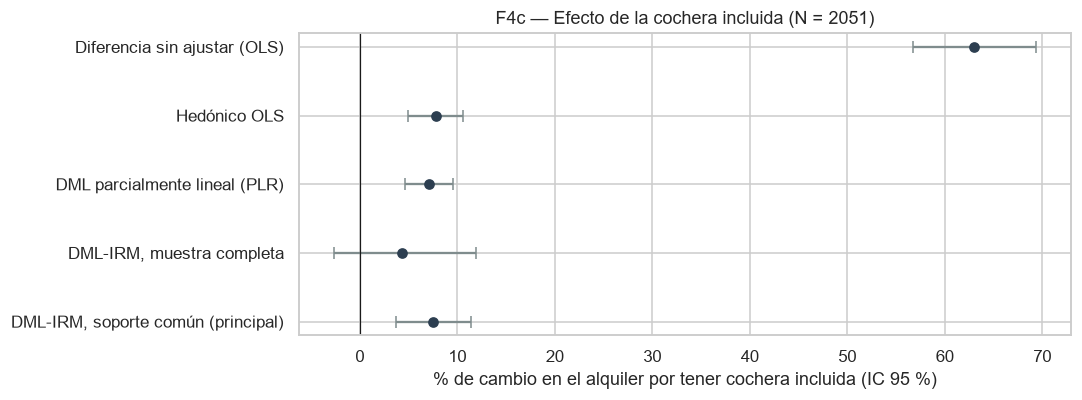
\includegraphics[width=0.85\textwidth]{F4c_estimadores_cochera.png}
\end{figure}

\textbf{Lectura}: casi todo el 63\,\% bruto era tamaño y zona. \textbf{H1 se confirma.} Aquí, a diferencia de los baños, la regresión lineal y Double ML coinciden. Sin el recorte al soporte común, el IRM se vuelve inestable (4.3\,\%, con un IC de $-2.7$ a 11.9\,\%), lo que muestra por qué el recorte es necesario.

\subsection{Qué decisiones importan (OE4, H2)}

\begin{itemize}
\item \textbf{Sin la ubicación}: 21.7\,\%, el efecto se triplica porque las cocheras abundan en los distritos caros.
\item Sin el área: 11.4\,\%. Sin baños ni dormitorios: 9.1\,\%.
\item \textbf{Con el precio por m²} (prohibido): $-0.5$\,\%.
\item Solo ``incluida'' explícita: 7.9\,\%. Contando también las cocheras de costo extra: 5.3\,\%, lo esperable porque su precio no las incluye.
\end{itemize}
\textbf{H2 se confirma.}

\subsection{¿Varía por zona? (OE4, H3)}

\begin{figure}[H]
\centering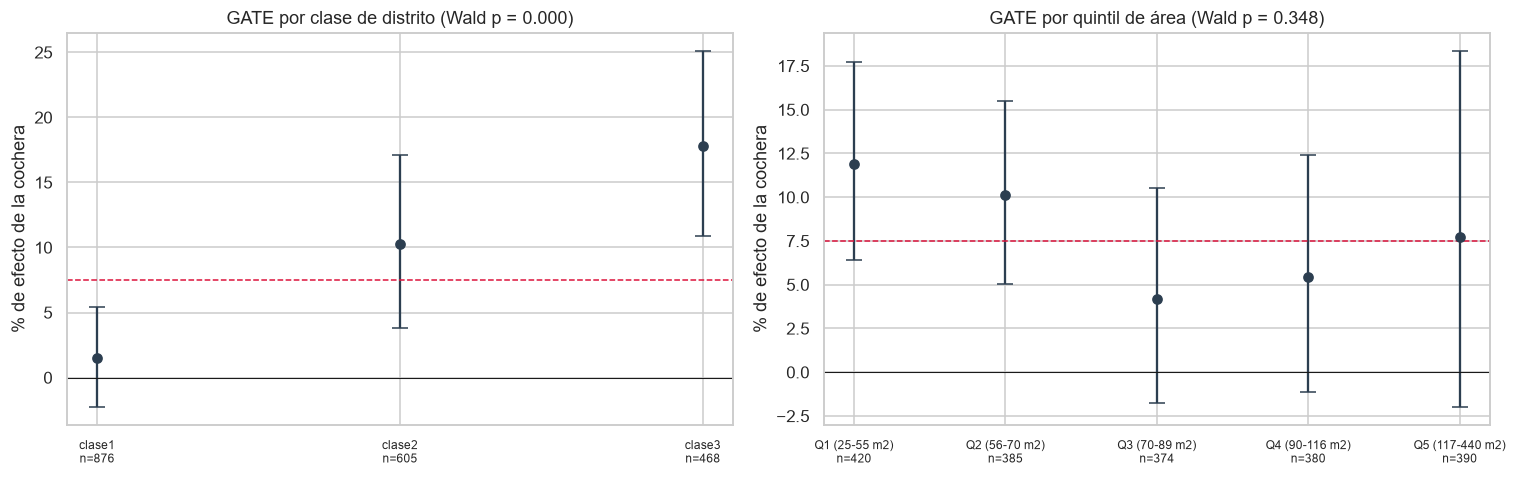
\includegraphics[width=\textwidth]{F7c_heterogeneidad_cochera.png}
\end{figure}

\textbf{Sí}: en Miraflores, San Isidro, Barranco y Lince la cochera casi no se paga (1.5\,\%, no significativo). En la clase2 vale 10\,\% y en la clase3 18\,\% (Wald $p=0.0001$). Una explicación posible, no probada: donde casi todos los avisos tienen cochera, no diferencia a uno de otro; donde escasea, se paga. Por tamaño no hay diferencias. \textbf{H3 se confirma para la cochera.}

\subsection{Qué tan frágil es (OE4, H4)}

\begin{itemize}
\item \textbf{RV = 0.105}: un factor oculto que explique el 10.5\,\% de la variación sobrante de la cochera \emph{y} del precio anularía el efecto.
\item Uno tan fuerte como la \textbf{antigüedad} lo dejaría en 0.4\,\%. Uno como la \textbf{ubicación} lo invertiría.
\item La simulación mostró que esta cota es \textbf{optimista} para el tratamiento binario: la fragilidad real podría ser mayor.
\end{itemize}
\textbf{H4 se confirma}: es un resultado \textbf{frágil}; vale bajo los supuestos del DAG.

\subsection{Baños (análisis secundario)}

Un baño adicional sube el precio \textbf{3.8\,\%} (1.7--6.0\,\%), unos S/\,100 al mes. Antes, con todas las direcciones, daba 5.3\,\%: \textbf{la ubicación imprecisa inflaba el efecto}. Controlar por la cochera lo deja en 3.5\,\%. No varía por zona y es igual de frágil.

\subsection{¿El método funciona? (OE6)}

\begin{table}[H]\small
\caption{Qué muestra la simulación}
\begin{tabularx}{\textwidth}{>{\raggedright\arraybackslash}p{3.6cm}L}
\toprule
Escenario & Resultado \\
\midrule
Cochera, nada oculto & Los tres métodos aciertan (cobertura 94--96\,\%). \\
Cochera, factor oculto & Todos se sesgan ($+0.04$) y la cota de sensibilidad lo \textbf{subestima}. \\
Baños, nada oculto & Double ML acierta (93\,\%); la regresión lineal se sesga. \\
Baños, factor oculto & Double ML se sesga, pero la cota \textbf{sí} lo detecta (95--98\,\%). \\
\bottomrule
\end{tabularx}
\end{table}

\subsection{Correspondencia con lo que pide tu asesor}

\begin{table}[H]\small
\caption{Requisitos de \texttt{nuevo\_informe} y dónde se cumplen}
\begin{tabularx}{\textwidth}{>{\raggedright\arraybackslash}p{4.6cm}>{\raggedright\arraybackslash}p{4.4cm}L}
\toprule
Requisito & Dónde & Estado \\
\midrule
Tratamiento binario bien definido & Cochera incluida (notebook 2b) & Hecho \\
R1 Auditoría y geografía & notebook 2 & Hecho \\
R2 Balance y soporte común & notebook 3b & Hecho \\
R3 Estimación primaria & notebook 3b & Hecho \\
R4 Especificaciones & notebook 3b (y 3 para baños) & Hecho \\
R5 Robustez a factores ocultos & notebook 3b & Hecho (cota optimista) \\
R6 Validación semisintética & notebook 4 & Hecho \\
R7 Heterogeneidad & notebook 3b & Hecho \\
R8 IA de medición & notebook 2b & Hecho; falta la validación humana \\
Figuras F1--F7 & \texttt{resultados/figuras} & Todas \\
Manuscrito y presentación & \texttt{informe/} & Hecho (65 págs.; 15 diapositivas) \\
Un comando que reproduzca todo & -- & Pendiente \\
\bottomrule
\end{tabularx}
\end{table}

\subsection{Cómo resumirlo en la defensa}

\begin{enumerate}
\item \textbf{Observacional}: con cochera, los avisos cuestan un 63\,\% más, pero casi todo es tamaño y zona.
\item \textbf{Causal (condicionado al DAG)}: tener cochera incluida sube el precio de oferta un 7.5\,\% (3.7--11.4\,\%), unos S/\,199 al mes.
\item \textbf{Hallazgo nuevo}: la cochera casi no se paga en los distritos más caros y se paga mucho donde escasea.
\item \textbf{Metodológico}: la IA mide la cochera por menos de 1 USD, y usar solo direcciones exactas cambia los resultados.
\item \textbf{Límite honesto}: un factor oculto como la antigüedad lo anularía, y falta validar la IA con etiquetas humanas.
\end{enumerate}

\subsection{Preguntas probables del jurado}

\begin{description}[leftmargin=0.4cm,style=nextline]
\item[¿Cómo sabes que la IA leyó bien la cochera?] Todavía no lo sé con certeza: el piloto corrigió errores evidentes y hay 249 avisos listos para la validación humana. Por eso el resultado se presenta como exploratorio.
\item[¿Y si un aviso tiene cochera pero no lo menciona?] Quedaría como ``sin cochera''. Si ese error es parejo entre zonas, achica el efecto: el real sería mayor.
\item[¿Por qué solo ROOFTOP?] Porque la ubicación es el confusor más importante. Con direcciones aproximadas, el control de la ubicación queda incompleto; de hecho, el efecto de los baños se inflaba.
\item[¿Por qué recortar a propensión 0.05--0.95?] Porque fuera de ese rango no hay departamentos comparables: el efecto solo podría extrapolarse. Sin recorte, el estimador se vuelve inestable.
\item[¿Por qué la cochera vale tan poco en Miraflores?] Hipótesis: allí la mayoría de la oferta ya la tiene y no diferencia un aviso de otro. No está demostrado.
\end{description}

% =====================================================================

\section{Glosario mínimo}\label{sec:glosario}

\begin{description}[leftmargin=0.4cm,style=nextline,itemsep=2pt]
\item[Tratamiento (T)] La variable cuyo efecto se mide: el número de baños.
\item[Resultado (Y)] Lo que se ve afectado: el logaritmo del precio.
\item[Confusor] Variable que causa a la vez el tratamiento y el resultado (el área). Hay que controlarla.
\item[DAG] Grafo de flechas ``A causa B'' que resume los supuestos causales.
\item[Criterio back-door] Regla para decidir qué controlar: bloquear todos los caminos no causales entre T e Y.
\item[Estimando] La cantidad exacta que se quiere estimar ($\theta$).
\item[Residuo] Lo que un modelo no logra explicar: valor real menos valor predicho.
\item[Double ML] Método que usa ML para quitar el efecto de los confusores al precio y al tratamiento, y luego relaciona los residuos.
\item[Cross-fitting] Predecir cada dato con modelos que no lo vieron al entrenar (como un cross-validation).
\item[p-valor] Probabilidad de ver un resultado así de extremo si no hubiera ningún efecto. Si es menor que 0.05, se llama ``significativo''.
\item[Intervalo de confianza (IC 95\,\%)] Rango de valores compatibles con los datos; un procedimiento que acierta el 95\,\% de las veces.
\item[Error estándar (EE)] Cuánto variaría la estimación con otra muestra.
\item[Errores agrupados] Errores estándar que reconocen que las observaciones de un mismo grupo (edificio o zona) no son independientes.
\item[$R^2$] Fracción de la variación de una variable que un modelo explica (0 a 1).
\item[Valor de robustez (RV)] Fuerza mínima de un factor oculto para anular el efecto.
\item[GATE] Efecto promedio calculado dentro de un grupo predefinido.
\item[Prueba de Wald] Prueba de si varios efectos son iguales entre sí.
\item[Potencia] Probabilidad de detectar un efecto que realmente existe.
\item[I de Moran] Medida de cuánto se parecen los valores de puntos cercanos en el mapa.
\item[Propensión] Probabilidad de recibir el tratamiento (tener cochera) dado el perfil del departamento.
\item[Soporte común] Zona de perfiles donde hay departamentos con y sin tratamiento para comparar (propensión entre 0.05 y 0.95).
\item[Balance / SMD] Qué tan parecidos son los grupos con y sin tratamiento; diferencia estandarizada menor que 0.1 = parecidos.
\item[IRM / AIPW] Double ML para tratamientos sí/no: combina la propensión y dos modelos del precio en un score doblemente robusto.
\item[ROOFTOP] Precisión de geocodificación de Google que indica el edificio exacto.
\item[Modelo de lenguaje (LLM)] Modelo de IA de texto (aquí \texttt{gpt-4.1-mini}) usado para leer las descripciones.
\item[Sesgo] Error sistemático: cuánto se equivoca un método en promedio.
\item[RMSE] Error típico de un método (combina el sesgo y la variabilidad).
\item[Cobertura] Porcentaje de veces que el IC contiene el valor verdadero (ideal: 95\,\%).
\item[Simulación semisintética] Usar datos reales pero inventar el resultado con un efecto conocido, para comprobar si el método lo recupera.
\end{description}

\end{document}
